
%-------------------------------------------------------------
%				RENDERED PRICES API
%-------------------------------------------------------------

\mcchap{API rendered prices}{cap:api}

Una volta implementati i vari Widget delle componenti delle homepage le specifiche di poter
modificare il contenuto delle componenti da interfaccia grafica e senza editare
il codice HTML, di poter creare copie delle componenti già create, e di poter spostare
semplicemente con drag and drop le varie componenti risultavano soddisfatte.

L'unico problema rimanente dunque era quello di avere un feedback visivo immediato durante l'editing della pagina.

Il feedback visivo era già presente per quelle componenti senza prodotti il cui HTML risiedeva in Wordpress,
per le componenti che fanno uso di prodotti invece l'utente che usava Wordpress non vedeva niente renderizzato.

Questo perchè una volta compilato il Widget, Wordpress renderizza il tag \emph{dynamic} e non i prodotti,
questi compaiono solo una volta che la pagina Wordpress viene processata da Kiruby, che trovando il tag \emph{dynamic}
lo sostituisce con l'HTML.

\begin{figure}
  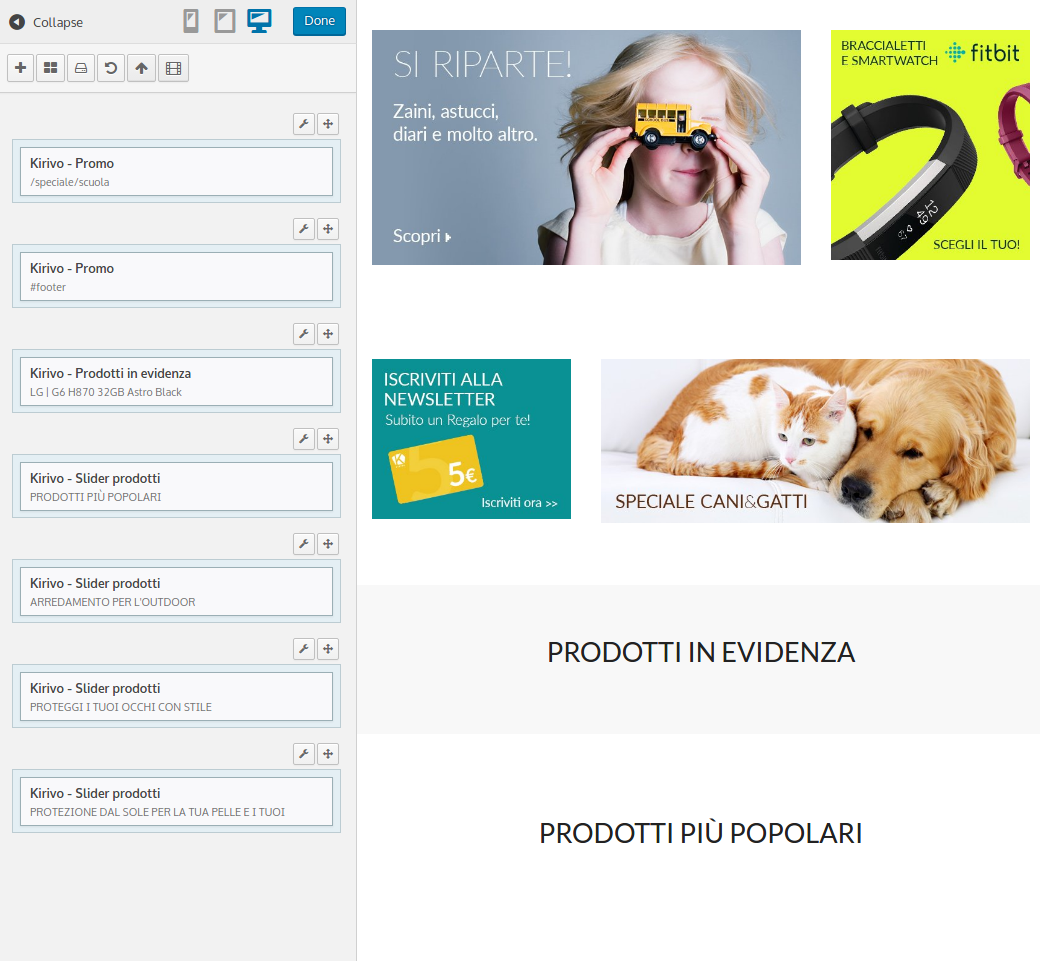
\includegraphics[width=\textwidth]{figure/noapi.png}
  \caption{Nella modalità di \emph{live editing} i prodotti non vengono visualizzati.}
  \label{fig:kspec}
\end{figure}

Per risolvere questa problema è stato deciso di implementare nel server Kiruby delle API chiamate
\emph{renderedAPI} che fatte delle richieste con gli ID dei prodotti e altri parametri come titolo e descrizione
ritorna il codice HTML con tutte le schede prodotto ed eventuali intestazioni.

Queste API poi vengono chiamate da Wordpress che riceve subito l'HTML e lo renderizza immediatamente,
le stesse API vengono anche chiamate da \emph{cmsdealer} per sostiture i tag \emph{dynamic}.

Per spiegare il meccanismo delle rendered API prendiamo in considerazione il meccanismo utilizzato per il Widget
\emph{Kirivo - Slider Prodotti} (vedi figura \ref{fig:smsrender}).

Altri Widgets come \emph{Origini - Slider Accessori}, \emph{Origini - Slider Prodotti} e \emph{Kirivo - Griglia Prodotti}
utilizzano un meccanismo praticamento identico ma utilizzano differenti template HTML.

\section{Creazione chiamata in Wordpress}
Innanzitutto per tutti quei Widget che fanno chiamate alle API è stata creata una superclasse PHP chiamata
\emph{AbstractProductWid}.
Qui nel metodo \emph{Widget}, che stampa l'HTML del Widget, viene stampato il contenuto che si riceve facendo la chiamata alle
API. L'indirizzo a cui viene fatta la chiamata viene composta con il metodo \emph{composeUrl}.

\begin{lstlisting}[style=customphp, language=Php,caption={I metodi Widget e \emph{callApiAndRender} di \emph{AbstractProductWid}}] 
function Widget($args, $instance){
	$this->callApiAndRender($this->composeUrl($instance));
}

function callApiAndRender($url) {
	$api_response = wp_remote_get($url);
	$api_data = json_decode( wp_remote_retrieve_body
		( $api_response ), true );
	echo str_replace('\n','',$api_data['rendered_html']);
}
\end{lstlisting}

Il metodo composeUrl della classe \emph{AbstractProductWid} inizia a comporre la chiamata con quei campi
comuni a tutti i Widget che fanno chiamate alle API ovvero: gli ID dei prodotti, e il titolo della sezione.

\begin{lstlisting}[style=customphp, language=Php,caption={Il metodo \emph{composeUrl} di \emph{AbstractProductWid}}] 
function composeUrl($instance) {
    $api_request = getHost();
    $api_request .= '/iguana/api/cms/' . $this->iguanaApiRoute() . 
    	'?product_ids=' . $instance['ids'];

    if(!is_null($instance['title'])) {
        $api_request .= "&title=".urlencode($instance['title']);
    }

    return $api_request;
}

\end{lstlisting}

Le classi che estendono \emph{AbstractProductWid} devono poi definire il metodo \emph{iguanaApiRoute}, che specifica
a quale rotta il Widget deve fare la chiamata ed eventualmente aggiungere campi alla chiamata, sovrascrivendo \emph{callApiAndRender} con la 
chiamata al metodo \emph{composeUrl} della superclasse come prima istruzione.

Ad esempio il codice del Widget \emph{Kirivo - Slider Prodotti} che deve fare la chiamata alla rotta \emph{/iguana/api/cms/rendered\_box\_prices} e aggiungere  anche i campi link allo \emph{scopri altro} e sottotitolo sarà:

\begin{lstlisting}[style=customphp, language=Php,caption={Viene sovrascritto \emph{iguanaApiRoute} da \emph{ProductsWidget} per specificare la chiamata da effettuare}] 
function iguanaApiRoute() {
    return 'rendered_box_prices';
}
\end{lstlisting}

\begin{lstlisting}[style=customphp, language=Php,caption={Ridefinendo \emph{composeUrl} vengono aggiunti ulteriori campi specifici del Widget \emph{ProductsWidget}}] 

function composeUrl($instance) {
  $api_request = parent::composeUrl($instance);
  if(!is_null($instance['subtitle'])) {
    $api_request .= "&subtitle=".urlencode($instance['subtitle']);
  }
  if(!is_null($instance['scopri-link'])) {
    $api_request .= "&link=". urlencode($instance['scopri-link']);
  }
  return $api_request;
}
\end{lstlisting}

\section{Creazione risposta in Kiruby}

Il Widget \emph{ProductsWidget} quindi, quando deve essere renderizzato, fa una chiamata del tipo
\begin{verbatim}
https://origini.it/iguana/api/cms/rendered_box_prices?product_ids=id1,id2,id3
&title=carouseltitle
\end{verbatim}
ne preveleva il contenuto e lo stampa.

Vediamo ora come sono state implementate le risposte in Kiruby.

Per implementare delle rotte bisogna estendere una classe già presente in Kiruby chiamata \emph{AbstractRoute}.

Dopodichè è stato creato un modulo chiamato \emph{RenderedCmsApiRouteModule} dove vengono implementati metodi comuni
a tutte le rotte delle renderedAPI, come l'estrazione del titolo, e la logica per splittare il valore passato nel
parametro product\_ids e da questo prendere le informazioni di tutti i prodotti.

\begin{lstlisting}[language=Ruby,caption={Il metodo \emph{title} che preleva il parametro \emph{title} se presente}] 
def title
    params[:title].present? ? params[:title] : ''
end
\end{lstlisting}

\begin{lstlisting}[language=Ruby,caption={Il metodo \emph{product\_ids} trasforma gli ids passati nel parametro in un array}] 
def product_ids
    params[:product_ids].gsub(/\s+/, '').split(',')
end
\end{lstlisting}

La risposta di una sottoclasse di \emph{AbstractRoute} viene implementata nel metodo \emph{response\_hash}, le rotte restiscono un JSON
così strutturato:
\begin{verbatim}
{rendered_html: "<section>....(conenuto html da renderizzare)..</section>"}
\end{verbatim}

\begin{lstlisting}[language=Ruby,caption={Il metodo \emph{response\_hash} dove viene creato il JSON da restituire}] 
def response_hash
  session = create_session
  prices = session.filter_by_code(product_ids).get_results
  prices = ordered_prices(prices)
  {rendered_html: rendered_html(prices, title, subtitle, link)}
end
\end{lstlisting}

Il metodo \emph{response\_hash}, preleva tutte le informazioni dei prodotti chiamando il metodo
\begin{verbatim}
session.filter_by_code(product_ids).get_results
\end{verbatim}
e il contentuo restituito dal JSON viene fornito chiamando il metodo \emph{rendered\_html}.

\begin{lstlisting}[language=Ruby,caption={Il metodo \emph{rendered\_html} restituisce il contenuto dell'erb compilato con i parametri passati con la chiamata FileTemplate.for\_kirivo}] 
def rendered_html(prices, title, subtitle, link)
  FileTemplate.for_kirivo('kirivo_products_box.erb', 
    OpenStruct.new({products: prices, title: URI.decode(title))
end
\end{lstlisting}

Una volta presi i prodotti vengono passati insieme al titolo all'erb \emph{kirivo\_products\_box.erb}, che a sua volta per ogni prodotto
compila l'erb \emph{products\_template.erb}.
\newpage
\begin{lstlisting}[basicstyle=\tiny,caption={Il template \emph{kirivo\_products\_box.erb}}] 
<section id="hp_specials" class="bg_white">
  <div class="row text-center">
    <h5 class="subheader text-center"><%= title %></h5>
  </div>

  <div class="row small-up-1 medium-up-3 large-up-4" data-equalizer="box_offer_height">
    <% products.each do |product| %>
        <%= FileTemplate.for_kirivo('product_template.erb', {price: product}) %>
    <% end %>
  </div>
</section>
\end{lstlisting}
\begin{lstlisting}[basicstyle=\tiny, caption={Il template \emph{products\_template.erb}}] 
<% price = model[:price] %>
<div class="columns product_tile end" data-price-container>
  <div class="deal_offer_tile" data-merchant-id="<%= price.merchant_id %>">
    <div class="feedback_mask">
      <a href="<%= Kirivo::ProductSheetRoute.url_for(price) %>">
        <div class="upper_tile">
          <div class="image_box">
              <picture>
                <img src="<%= price.image_url_for(300) %>"%>"/>
              </picture>
          </div>
        </div>
      </a>
      <div class="bottom_tile">
        <div class="tile_description">
          <small class="tile_quantity text_grey"><%= price.capacity %></small>
          <a href="<%= Kirivo::ProductSheetRoute.url_for(price) %>">
            <h4 class="product_name" data-price-name>
              <strong><%= price.name %><% if price.is_year_defined %>
            <% end %>
            </strong></h4>
          </a>
        </div>
      </div>
      <div class="cart_feedback">
        <i class="fa fa-3x fa-check"></i>Aggiunto al carrello
      </div>
    </div>
    <div class="tile_hover">
      <form class="add_to_cart_form" action="<%= Cart.add_to_cart_url %>" method="post">
        <button id="add_to_cart_<%= price.id %>" class="button_add_to_cart" data-add_to_cart>
          <i class="fa fa-shopping-cart"></i> AGGIUNGI AL CARRELLO
        </button>

        <input name="qty" class="qty" value="1" type="hidden">
        <input name="productCodePost" value="<%= price.id %>" type="hidden" data-price-id>
      </form>
      <input name="ean" value="<%= price.ean_codes.first %>" type="hidden" data-price-ean>
    </div>
  </div>
</div>
\end{lstlisting}


\begin{figure}
  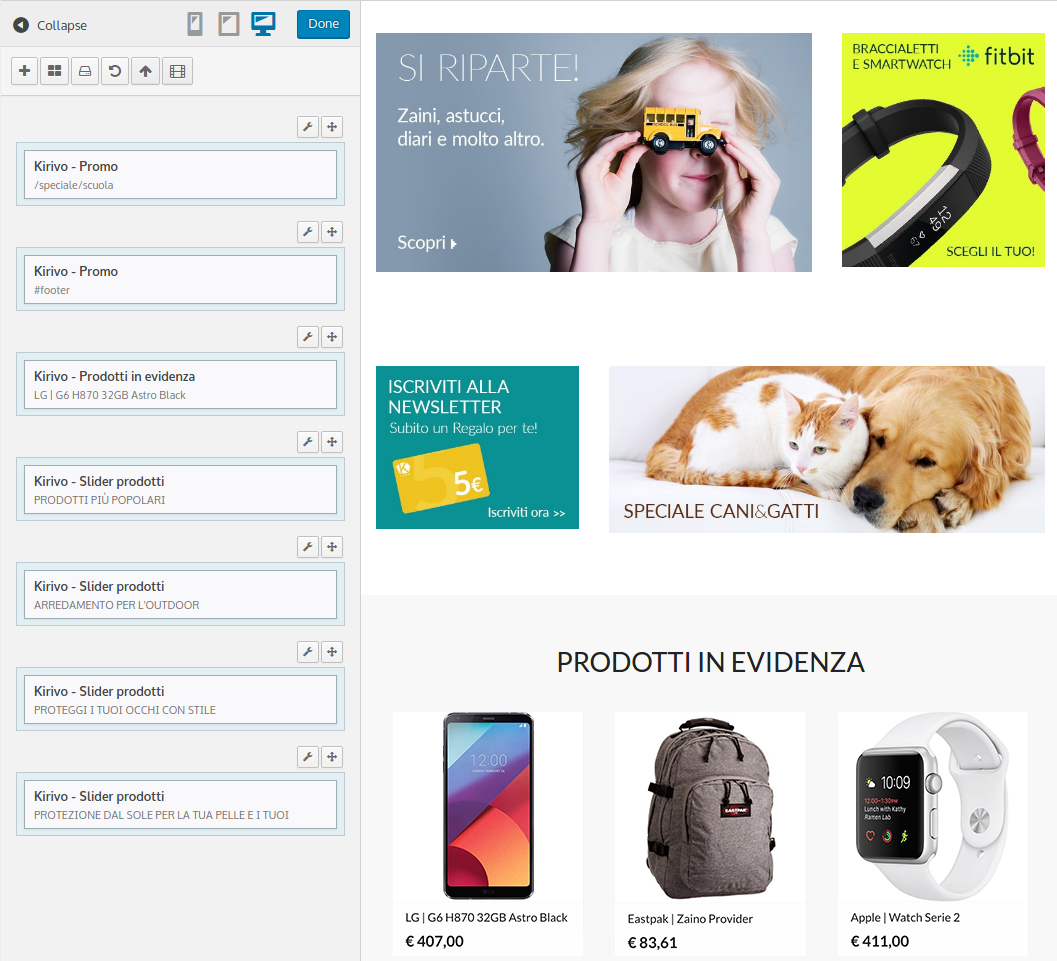
\includegraphics[width=\textwidth]{figure/livedit.png}
  \caption{Con le renderedAPI, in modalità \emph{live edit}, i prodotti vengono visualizzati.}
  \label{fig:kspec}
\end{figure}

\newpage
\section{Creazione chiamata in cmsdealer}

La gemma \emph{cmsdealer} per trasformare i dynamic tag in contenuto renderizzato usava una procedura simile 
a quella delle renderedAPI, con la differenza che invece dei parametri della chiamata venivano letti i parametri
del tag \emph{dynamic}, e invece che restituire l'HTML della componente in un JSON questo veniva direttamente
scritto nella pagina dove veniva letto il tag \emph{dynamic}.

Nonostante la creazione delle renderedAPI, \emph{cmsdealer} veniva ancora utilizzato,
questo perchè nei siti a parte le homepage ci sono ancora pagine compilate scrivendo direttamente l'HTML
e che usano i dynamic tag.

Per evitare duplicazione di codice, in particolare la presenza doppia degli \emph{erb} dei template dei prodotti,
si è fatto in modo che quando \emph{cmsdealer} legge un tag \emph{dynamic}, sostituisce questo con il contenuto
che viene restituito dalle renderedAPI.

Per fare questo, in modo simile ai Widget, è stata implementata una sottoclasse di \emph{DynamicTag} chiamata
\emph{ApiCallingTag}.

In questa classe viene implementato il meccanismo di composizione della chiamata, la lettura della risposta e la sostituzione 
del contenuto di quest'ultima con il tag \emph{dynamic}.

Il metodo che restituisce il contenuto da sostituire \emph{replaced\_html} è stato ridefinito in modo da ritornare
il contenuto della risposta delle API.

\begin{lstlisting}[language=Ruby,caption={Il codice della classe \emph{ApiCallingTag}}] 
class ApiCallingTag < DynamicTag
  def replaced_html(original_url = nil)
    params = {url: original_url}
    allowed_api_parameters.each do |p|
      params[p] = eval(p) if self.respond_to?(p)
    end
    json = JSON.parse(Connection.new.get(url_for(params)).body)
    json['rendered_html']
  end

  def url_for(params)
    URI.add_params("www.origini.it/iguana/api/cms/#{get\_route}",
     params)
  end
end
\end{lstlisting}

Le sottoclassi di \emph{ApiCallingTag} invece devono implementare due metodi ovvero \emph{get\_route},
dove viene definito quale rotta delle renderedAPI chiamare, e \emph{allowed\_api\_parameters} dove viene definita
un array con i parametri che possono essere letti dal tag \emph{dynamic}.

Per esempio il dynamic tag OriginiListingBox quando legge il tag può individuare ed inoltrare nella chiamata i parametri
product\_ids, title, description, number, listing\_link e aggiungerà questi parametri alla chiamata alla rotta: 

\emph{www.origini.it/iguana/api/cms/rendered\_origini\_listing\_box}

\begin{lstlisting}[language=Ruby,caption={Il codice della classe che legge e trasforma il tag con type \emph{OriginiListingBox}}] 
class OriginiListingBox < ApiCallingTag
  def allowed_api_parameters
    ['product_ids','title','description', 'number','listing_link']
  end

  def get_route
    'rendered_origini_listing_box'
  end
end
\end{lstlisting}

\emph{Cmsdealer} quindi quando troverà un tag del tipo
\begin{verbatim}
<dynamic type="OriginiListingBox" product_ids="id1,id2,id3" title="products" 
  listing_link="/speciale/spedizione_gratuita">
\end{verbatim}
Sostituirà a questo il contenuto ritornato dalla chiamta alla rotta
\begin{verbatim}
www.origini.it/iguana/api/cms/rendered_origini_listing_box&product_ids=id1,id2,id3
&title=products&listing_link=%2Fspeciale%2Fspedizione_gratuita\end{verbatim}

Così facendo tutti i requisiti del progetto risultano soddisfatti.
Nei due capitoli successivi vengono elencati i Widget creati per i due siti, specificando
quali valori sono stati resi personalizzabili.
